\chapter{Training, Testing and Hyperparameters Tuning of a Multi-class
Vehicle Classifier}
\label{Chapter 4}
As mentioned in earlier chapters, CNNs are predominantly used for
image classification and detection in pattern recognition and
computer vision problems. Recall that classification is the process of putting a tag on
an image from a set of class labels. This chapter describes in detail
the process of designing, training, testing and hyper-parameters
tuning of a a five-class image classifier. The following sections
cover in detail the step-by-step process of training a five-class vehicles
classifier. Furthermore, results are tabulated as values of
hyper-parameters are changed to achieve better test accuracy and reduced
classification loss. An overview of the system is given in
Figure \ref{system_overview}.

\begin{figure}
    \centering
    \captionsetup{justification = centering}
    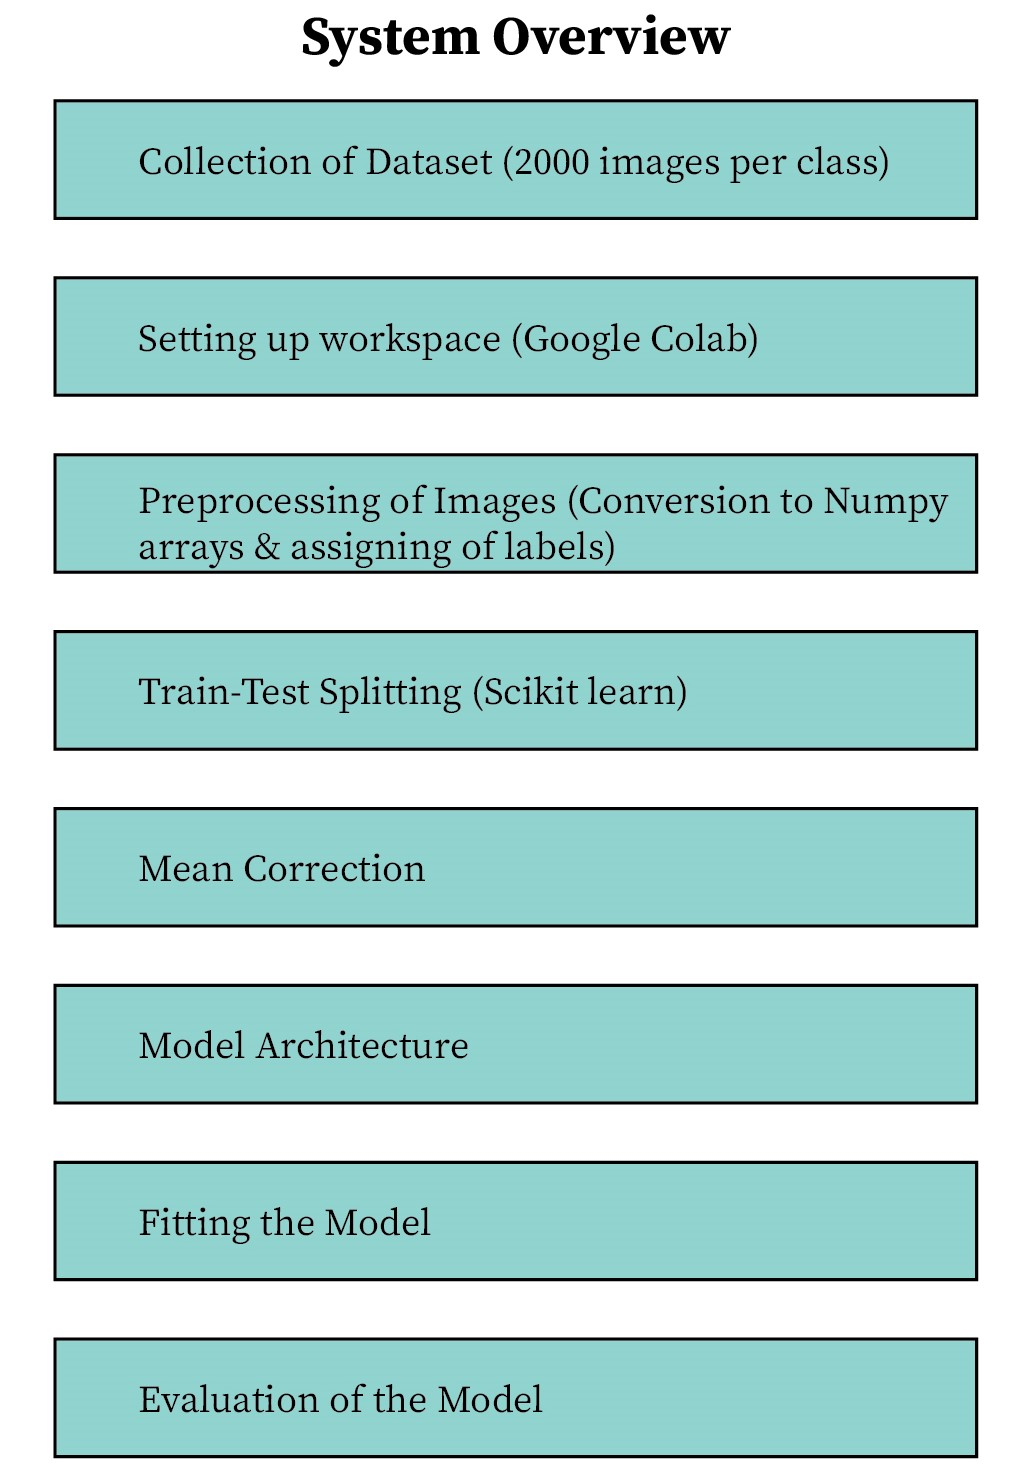
\includegraphics[scale = 0.9]{CHAPTERS/Chapter-4/Images/system_overview-01.jpg}
    \caption{System overview for a multi-class vehicles classifier  } 
    \label{system_overview}
  \end{figure}
\section{Formation of Dataset}
Deep learning based image classification works by inputting class
image examples to a CNN; CNN is then trained for higher test accuracy
and reduced test loss. The set of images used for this purpose is
called a dataset.
The dataset is divided into training and test dataset by a specific ratio.
In this project we have five different classes of vehicles i.e. Bus, Car, Truck, Motorcycle
and Hiace. There are a total of 10000 images with 2000 images of each 
class. These images are downloaded from Google search results and from already available
datasets and from websites providing licensed free images like Flickr.
APIs along with Python
scripts can be used to download these images from the internet.
Using matplotlib in python, we can plot some of the images with the output as
shown in listing \ref{listing:4.1} and plot is attached in figure
\ref{fig:4.1}.
\linespread{1.0}
\begin{listing}[H]
\begin{minted}[bgcolor=bg,
    linenos = true,
    xleftmargin=20pt,
    framesep = 2mm]{python}
import matplotlib.pyplot as plt
from matplotlib.image import imread  
path  = './images/'
for i in range(9):
    plt.subplot(330+1+i)
    filename = path + 'image_'+ str(i) + '.jpg'
    image = imread(filename)
    plt.imshow(image)    
    plt.show()
\end{minted}
\caption{Python script to plot some images from each class}
\label{listing:4.1}
\end{listing}

\begin{figure}[H]
    \centering
    \captionsetup{justification = centering}
    \includegraphics[scale = 0.8]{CHAPTERS/Chapter-4/Images/4.1.png}
    \caption{Plot of some images from each class} 
    \label{fig:4.1}
  \end{figure}

\subsection{Data Augmentation}
Training deep learning CNN architectures on larger datasets
results in more skillful models and improved classification accuracy.
However, availability of large amount of  class-specific data is a challenge.
This problem of lack of sufficient data can be solved using
techniques which expand the size of available data by introducing
modifications and variations by performing image manipulation.
Dataaugmentation is the process of applying techniques like shifting, 
flipping, rotating and varying the brightness etc on images to
introduce variations in images. The Keras deep learning NN library uses
ImageDataGenerator
class to achieve image data augmentation and is used in our code.

\section{Setting of Workspace for the Project}
There are a lot of images to be processed. To process images, high end GPU is
needed. Due to unavailability of an Nvidia GPU on the system, we used Google Colab.
It is an online platform having high end GPUs free provided by Google for training
up to 12 hours. Enabling a GPU in the notebook settings can accelerate the process of
training.
\section{Designing and Training of DCNN for Multi-Class Classification}
In our project we have used Keras for designing, training and testing of 
DCCN architectures for our multi-class classification problem.
Keras is one of the leading high level API for neural networks. It contains
many modules such as layers, cost functions, activation functions, initialization
schemes and regularization schemes. This project uses Keras for training purposes.
\subsection{Conversion of Images and Labels to Numpy Arrays}
After importing all the necessary packages, we are all set to pre-process our data.
Recall to chapter 2, where we studied the basics of an image. In Keras, an image has two
representations i.e. (width, height, color\_channels) and (color\_channels, width, height).
First approach is called as ``channels first approach" and
the latter is called as ``channels last approach".
We will use the ``channels last approach".

First step is to read the images from the folder mounted from Google drive.
Labels are assigned to classes from 0 to 4. Keras load\_img() routine loads image
from the folder with given target size. Target size for this project is chosen as
$128 \times 128$. This means that both width and height has a size of 128 pixels.
There are 3 color channels for RGB images. Images are then converted to numpy arrays using
Keras img\_to\_array() method. Labels are stored as 0, 1, 2, 3, 4 based on the class of image (as data is renamed).
Figure \ref{fig:class_labels} shows all the classes and corresponding labels.

\begin{figure}[H]
    \centering
    \captionsetup{justification = centering}
    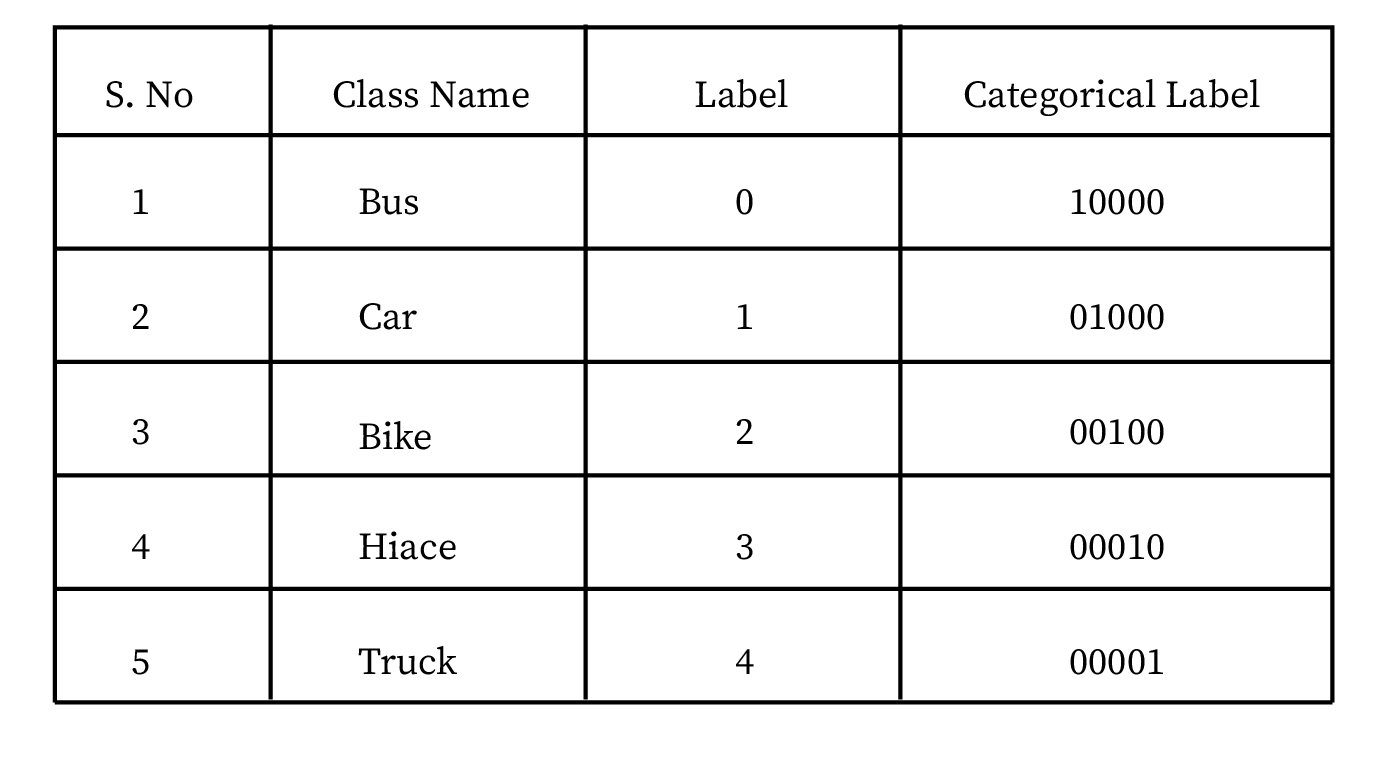
\includegraphics[scale = 0.2]{CHAPTERS/Chapter-4/Images/class_label-01}
    \caption{Classes and labels} 
    \label{fig:class_labels}
  \end{figure}

\noindent A section of code for this implementation is shown in listing \ref{listing:4.2}.

\begin{longlisting}
    \begin{minted}[bgcolor=bg,
        linenos = true,
        xleftmargin = 20pt,
        framesep = 2mm]{python}
folder = '/content/Input_data/'
images = np.zeros((num_of_images,img_rows,img_cols,color_channels))
labels = np.zeros(num_of_images)
i = 0
# enumerate files in the directory
for file in os.listdir(folder):
# determine class
    if file.startswith('bus'):
        output = 0
    elif file.startswith('car'):
        output = 1
    elif file.startswith('bike'):
        output = 2
    elif file.startswith('hiace'):
        output = 3
    else:
        output = 4
    # load image
    img = load_img(folder + file, target_size=(img_rows,img_cols))
    # convert to numpy array
    img = img_to_array(img)
    # store
    images[i] = img
    labels[i] = output
    i = i+1
\end{minted}

\caption{Conversion of Images to Numpy arrays}
\label{listing:4.2}
\end{longlisting}
In the code listing above ``images" on line 23, is a 4D tensor with
dimensions (10000, 128, 128, 3) which means that there are 10000
images with each image having $128\times 128\times 3$ matrices i.e.
each image has height and width of 128 pixels and 3 RGB channels in a
3D concurrent space. Also ,in the code listing above,
``labels", on line 24, is a 1D tensor containing the labels
for all the 10000 images available in our dataset.
\subsection{Train-Test Division}
In order to proceed with our DCNN multi-class classification model,
we need to split our available dataset into two parts, namely test 
dataset and train dataset. Both datasets have to be mutually-exclusive.
The train dataset is used for training our designed CNN.
Training involves three steps; feed forward, back propagation and
updation of model parameters. Test dataset is used to evaluate the performance
of our trained model on unseen data. Testing is a single step process
comprising of feed-forward only and it results in a  class
prediction for the input image. We used a ratio of 75\% and
25\% for train and test datasets respectively. The package used for this purpose is the
Scikit-learn train\_test\_split. Listing \ref{listing:4.3} shows splitting of
data into train and test.

\begin{listing}[H]
    \begin{minted}[bgcolor=bg,
        frame = lines,
        framesep = 2mm]{python}
train_images, test_images, train_labels, test_labels = 
train_test_split(images, labels, test_size = 0.25, random_state = 42)
\end{minted}
\caption{Train-test split}
\label{listing:4.3}
\end{listing}
There is another technique for splitting of data. In this technique, we make two directories,
namely, train and test and we randomly divide the images into these directories and then
convert them into numpy array. We have first converted the images
into arrays, split them into train and test and then we can save them back into
directories by converting them into images from array using PIL from\_array
function.

\subsection{Mean Correction}
After converting to float 32 and normalizing by 255, we have to subtract mean pixel.
Listing \ref{listing:4.4} illustrates the mean correction.

\begin{listing}[H]
    \begin{minted}[bgcolor=bg,
        linenos = true,
        xleftmargin = 20pt,
        framesep = 2mm]{python}
train_images = train_images.astype('float32') / 255
test_images = test_images.astype('float32') / 255

if subtract_pixel_mean:
    x_train_mean = np.mean(train_images, axis=0)
    train_images -= x_train_mean
    test_images -= x_train_mean

train_labels = to_categorical(train_labels,num_classes)
test_labels = to_categorical(test_labels,num_classes)
    \end{minted}
    \caption{Mean correction}
\label{listing:4.4}
\end{listing}
\noindent Lines 9 \& 10 shows the categorical labeling for using labels fit for Keras.
\subsection{CNN Model Architecture for Multi-Class Classification}
Recall from chapter \ref{Chapter 3}, a CNN model consists of various layers including
conv2D, Activation, MaxPoooling2D, Flatten and Dense layer.
Block diagram of the model architecture is shown in Figure \ref{fig:model_summary_2}. 
\begin{figure}[H]
    \centering
    \captionsetup{justification = centering}
    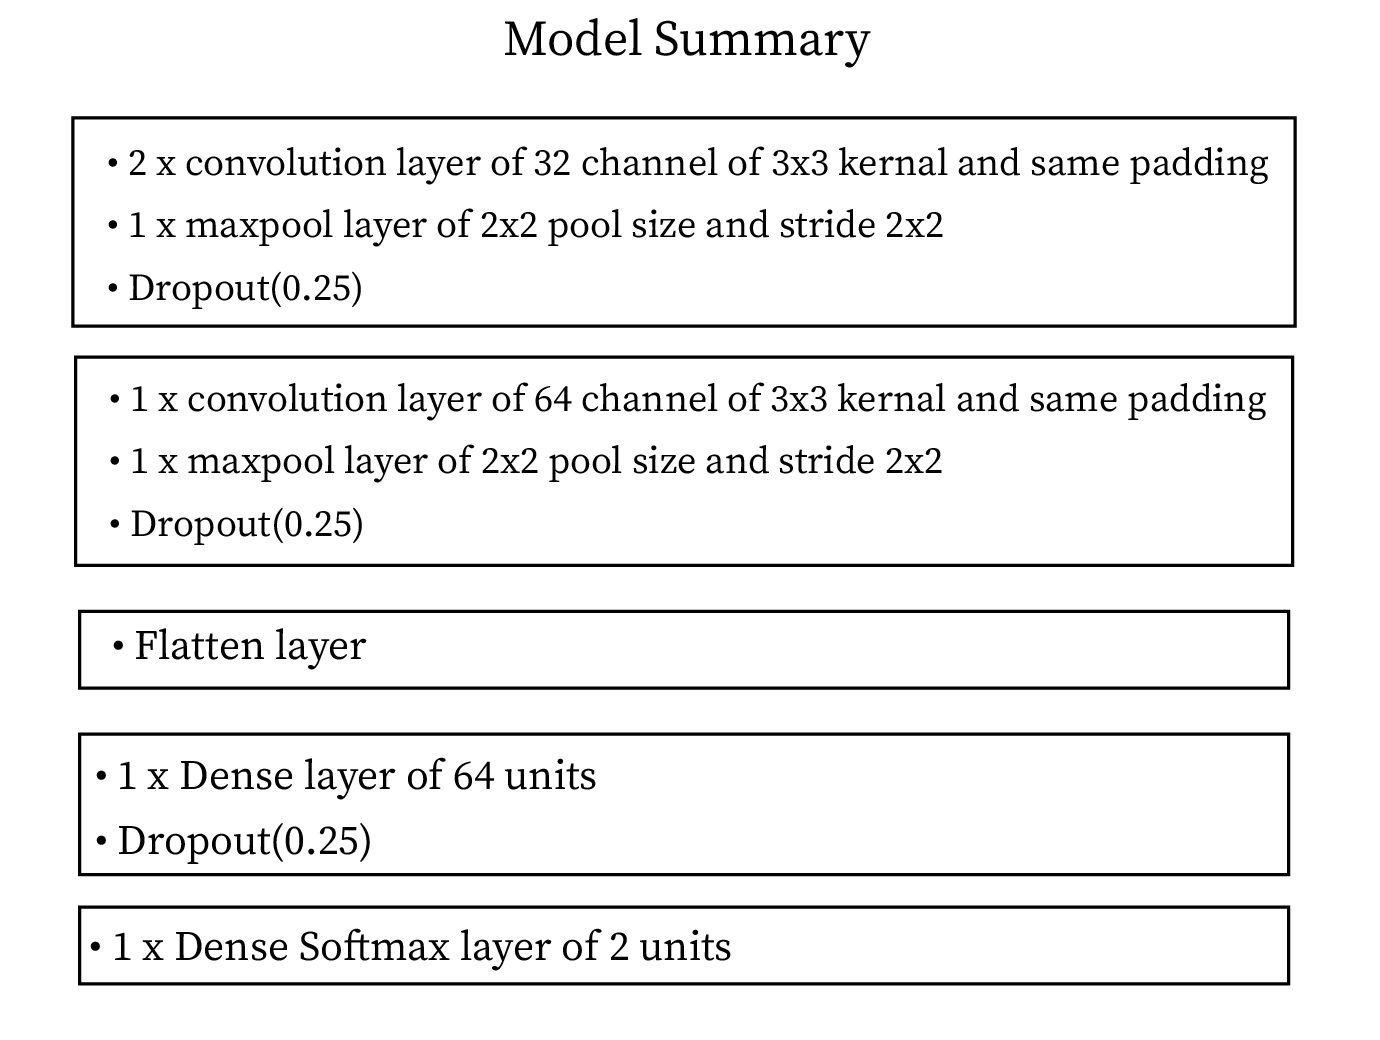
\includegraphics[scale = 1]{CHAPTERS/Chapter-4/Images/model_summary_2}
    \caption{Model architecture for binary class vehicle classifier} 
    \label{fig:model_summary_2}
\end{figure}
\noindent Listing \ref{listing:4.5}
defines the the architecture of our CNN Model.
\begin{longlisting}
    \begin{minted}[bgcolor=bg,
        linenos = true,
        xleftmargin = 20pt,
        framesep = 2mm]{python}
#Model
model = Sequential()
model.add(Conv2D(32, (3, 3), padding='same', activation = "relu",
                         input_shape=train_images.shape[1:]))
model.add(Conv2D(32, (3, 3), activation = "relu"))
model.add(MaxPooling2D(pool_size=(2, 2)))
model.add(Dropout(0.25))   

model.add(Conv2D(64, (3, 3), padding='same', activation = "relu"))
model.add(MaxPooling2D(pool_size=(2, 2)))
model.add(Dropout(0.25)) 
     
model.add(Flatten())

model.add(Dense(64))
model.add(Activation('relu'))
model.add(Dropout(0.5)) 

model.add(Dense(num_classes))
model.add(Activation('softmax'))

model.compile(loss='categorical_crossentropy', optimizer='adam',
metrics=['accuracy'])
    \end{minted}
    \caption{Defining the Model}
\label{listing:4.5}
\end{longlisting}
\noindent Lines 22 \& 23 define the loss function,
optimizer type and evaluation metrics used for training our CNN.
\subsubsection{Loss Function}

For more than two classes, loss is categorical\_crossentropy. For two
classes it is binary\_crossentropy. There are many optimizers in Keras i.e.
SGD, Adam, RMSprop, Adamax etc. Here we have used Adam. Accuracy metrics calculates how
often prediction equals labels.
\subsection{Fitting the Model}
Here the process of training starts. We have two functions used in Keras. One
is `model.fit' and other is `model.fit\_generator'. We have implemented data augmentation using a\
in our code using an if-else logic. We have also defined a validation set.
Validation data evalautes the behavior of the trained model to an unseen data.

An `epoch' is defined as a ``complete pass over an entire dataset" during the training process.
We have to determine the specific number of epochs for which the training process has to
run. If we pass over the entire dataset too many times,
it may result it increased training accuracy and reduced training loss
but it may also result in reduced validation accuracy and higher validation loss.
This specific scenario where validation accuracy is lower
than training accuracy or validation loss is higher  than
training loss is called ``overfitting''. Over-fitting means that our
CNN model has actually memorized the training examples or ``seen data"
instead of learning discernable parameters from it,
and it will not work well on `unseen data'. We have to avoid the overfitting. For this we have to search for
optimum values hyper-parameters of or model such as epochs,
batch size, optimizers, convolutional layers,
layer filters,filter sizes, drop-out layers etc.
Listing \ref{listing:4.6} shows the code for training process.

\begin{longlisting}
    \begin{minted}[bgcolor=bg,
        linenos = true,
        xleftmargin = 20pt,
        framesep = 2mm
        ]{python}
if not data_augmentation:
    print('Not using data augmentation.')
    history = model.fit(train_images, train_labels, validation_data =
    (test_images, test_labels), batch_size = batch_size, epochs = n_epochs)
else:
    datagen = ImageDataGenerator(
        zca_epsilon=1e-06,
        rotation_range=0,  
        width_shift_range=0.1,
        height_shift_range=0.1,
        shear_range=0.,
        zoom_range=0.,
        channel_shift_range=0.,
        fill_mode='nearest',
        cval=0.,
        rescale=None,
        preprocessing_function=None,
        data_format=None,
        validation_split=0.0)
    
    datagen.fit(train_images)
    
    history = model.fit_generator(datagen.flow(train_images, train_labels,
    batch_size = batch_size),validation_data=(test_images, test_labels),
    epochs = n_epochs)    
    \end{minted}
    \caption{Training the Model}
\label{listing:4.6}
\end{longlisting}
\subsection{Plotting the Accuracy and Loss}
A specific model with  chosen values of hyper-parameters
generates a specific accuracy upto which it can classify unseen data
Increasing epochs will not increase the accuracy, it basically overfits
the model. For a certain model, we have to find a specific number
of epochs. For this we plot the accuracy and loss of training and
validation data. Listing \ref{listing:4.7} shows the script for plotting the accuracy and
loss of training and validation data.

\begin{longlisting}
    \begin{minted}[bgcolor=bg,
        linenos = true,
        xleftmargin = 20pt,
        framesep = 2mm
        ]{python}
plt.grid()
plt.plot(history.history['accuracy'])
plt.plot(history.history['val_accuracy'])
plt.title('model accuracy')
plt.ylabel('accuracy')
plt.xlabel('epoch')
plt.legend(['train', 'validation'], loc='upper left')
plt.show()
# summarize history for loss
plt.grid()
plt.plot(history.history['loss'])
plt.plot(history.history['val_loss'])
plt.title('model loss')
plt.ylabel('loss')
plt.xlabel('epoch')
plt.legend(['train', 'val'], loc='upper left')
plt.show()
\end{minted}
\caption{Training, validation accuracy \& loss vs. epochs}
\label{listing:4.7}
\end{longlisting}

\subsection{Saving Model \& Weights}
After successful training of model, we have to resuse it
at evaluation or testing time. For this, the trained model is saved to our disk.
At testing time, this model can be loaded into Keras 
from our workspace. The Model is stored as .h5 file in the root directory.
Listing \ref{listing:4.8} shows the script for saving the weights.

\begin{listing}[H]
    \begin{minted}[bgcolor=bg,
        linenos = true,
        xleftmargin = 20pt,
        framesep = 2mm
        ]{python}
# Save model and weights
if not os.path.isdir(save_dir):
    os.makedirs(save_dir)
model_path = os.path.join(save_dir, model_name)
model.save(model_path)
print('Saved trained model at %s ' % model_path)
\end{minted}
\caption{Saving the Model}
\label{listing:4.8}
\end{listing}
\section{Evaluation of Model}
Evaluation of  the trained model over test dataset is  performed in two steps.
In the first step, the pre-trained model is loaded from the workspace.
In second step, `evaluate' function is used to run the run testing
phase on the test data. The function takes
test images and labels of the test images as input and, in turn,
generates a class label prediction for the input  test image. Listing \ref{listing:4.9} shows the script for
evalaution.
\begin{longlisting}
    \begin{minted}[bgcolor=bg,
        linenos = true,
        xleftmargin = 20pt,
        framesep = 2mm
        ]{python}
#Load Model
loaded_model = load_model("saved_models/model.h5")
#Evaluate Model
test_loss, test_acc = loaded_model.evaluate(test_images, test_labels)
print('Accuarcy of the model:', test_acc)
\end{minted}
\caption{Evaluating the Model}
\label{listing:4.9}
\end{longlisting}
\subsection{Two Class Problem \& Results}
We started with two class problem, Bus \& Car and recorded the results from 5
to 30 epochs.
The loss was binary\_crossentropy in this case. 
The training accuracy recorded after 25 epochs was 95.77\% and training
loss was 0.1269. The test set was choosen as validation data and validation accuracy after 5 epochs 
was 95.40\% and validation loss was 0.1271.
After 25 epochs for this model, the validation loss increases which indicate
that we have to train that model up to 20 epochs. The values of training
and validation accuracy \& training and validation loss
against number of epochs for binary class vehicle classifier
are tabulated in Table \ref{table:4.1}.
\begin{table}[H]
    \caption{Results for binary class vehicle classifier}
    \label{table:4.1}
	  \begin{center}
		\scalebox{0.85}
		{\begin{tabular}{|l |l |l |l |l |l |}
		\hline
		S.No & Number of epochs & Training accuracy & Validation accuracy & Training loss & Validation loss\\ \hline
		1  & 5 & 0.8783 & 0.9140 & 0.3083 & 0.2398
		\\ \hline
		2  & 10 & 0.9040 & 0.9440 & 0.2538 & 0.1585 
		\\ \hline
		3   & 15 & 0.9197  &  0.9410 & 0.2029 & 0.1652
        \\ \hline %
        4   & 20 &  0.9513 & 0.9650  &0.1408  & 0.0882
        \\ \hline %
        5   & 25 &  0.9577 & 0.9540  &0.1269  & 0.1271
        \\ \hline %
        6   & 30 &  0.9593 & 0.9550  &0.1126  & 0.1337
		\\ \hline %
		\end{tabular}}
	  \end{center}
\end{table}
\noindent The plot of training and validation accuracy and training and validation
losses for 30 epochs are plotted using Python matplotlib shown in figure \ref{fig:4.4}.
\begin{figure}[htbp]
    \centering
    \begin{subfigure}[t]{0.45\textwidth}
        \fbox{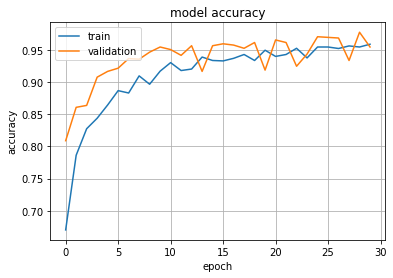
\includegraphics[scale = 0.5]{CHAPTERS/Chapter-4/Images/4.4a}}
        \caption{Training \& validation accuracy}
        \label{fig:4.4a}
    \end{subfigure}
    \begin{subfigure}[t]{0.45\textwidth}
        \fbox{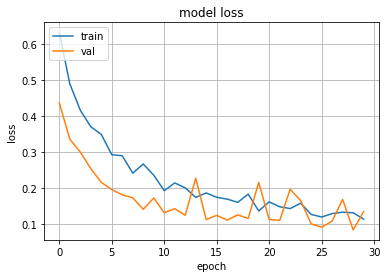
\includegraphics[scale = 0.5]{CHAPTERS/Chapter-4/Images/4.4b}}
        \caption{Training \& validation loss}
        \label{fig:4.4b}
    \end{subfigure}
    \caption[]{Model accuracy \& model loss}
    \label{fig:4.4}
  \end{figure}


\subsection{Five Class Probem \& Results}
We started with two class problem and extended the model to five classes
which is our desired task. The loss function in this case is categorical\_crossentropy.
The model used for five class is a customized VGG-16. The details of the
model are shown in figure \ref{model_summary}.
\begin{figure}[H]
    \centering
    \captionsetup{justification = centering}
    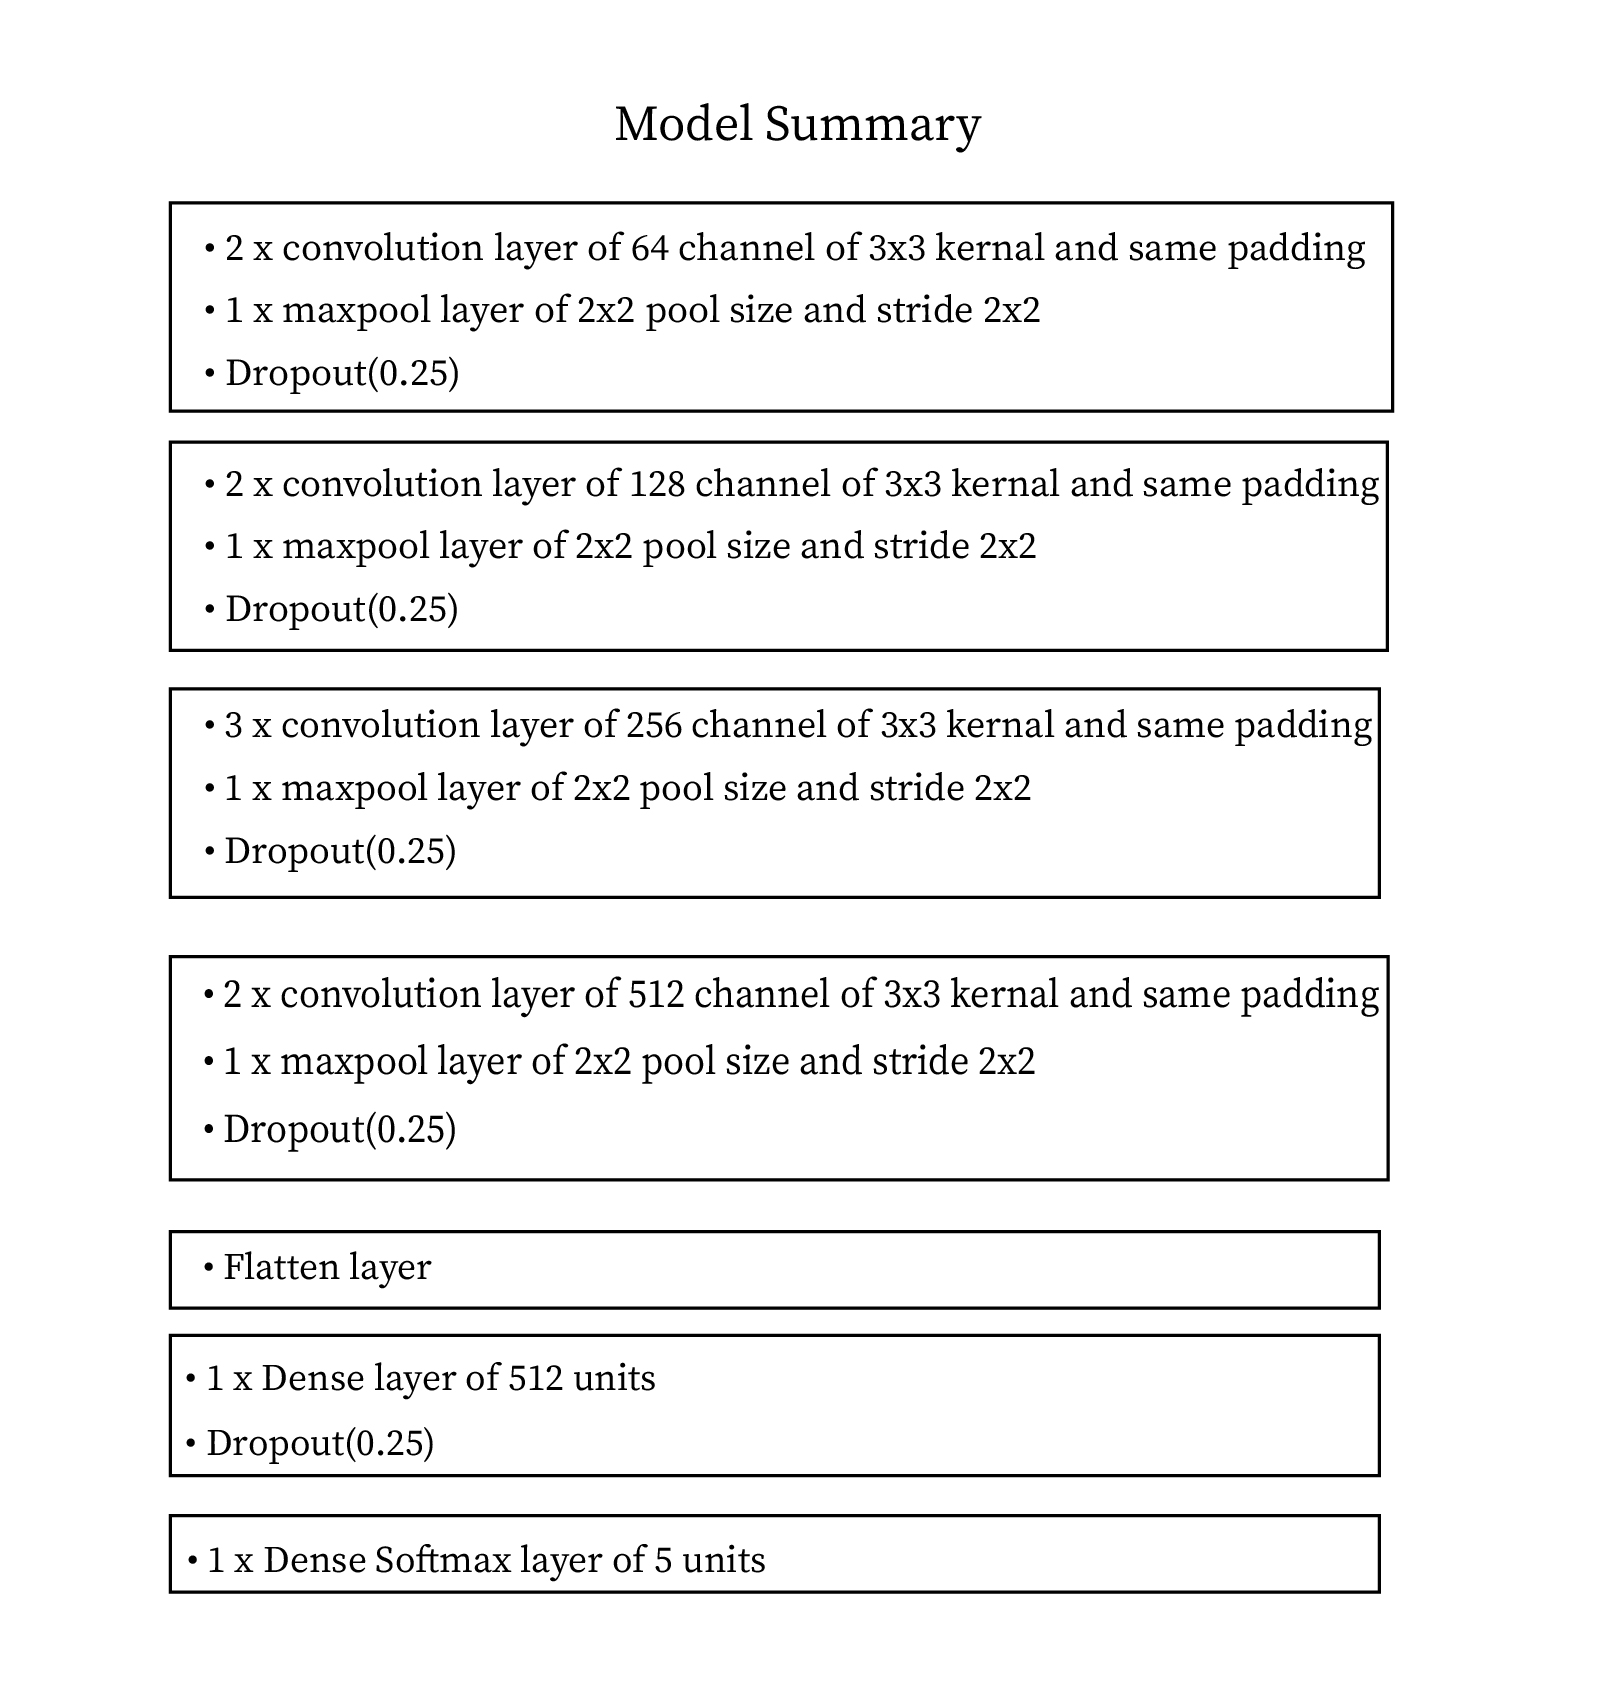
\includegraphics[scale = 0.8]{CHAPTERS/Chapter-4/Images/summary.jpg}
    \caption{Model architecture for five class vehicle classifier} 
    \label{model_summary}
\end{figure}
\noindent The optimizer used is RMSprop with
learning rate 0.0001. We started with 5 epochs, then 10 upto 20. The plot of training
and validation accuracy and training and validation loss is plotted using Python
matplotlib and it is observed that near to 20 the validation loss
increases and validation accuracy decreases. So we stopped at 20 epochs
and recorded the results. The plots are shown in
figure \ref{fig:4.6}.
\begin{figure}[htbp]
    \centering
    \begin{subfigure}[t]{0.45\textwidth}
        \fbox{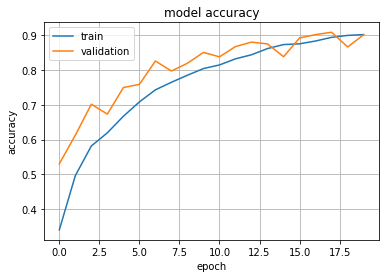
\includegraphics[scale = 0.5]{CHAPTERS/Chapter-4/Images/4.6a}}
        \caption{Training \& validation accuracy}
        \label{fig:4.4a}
    \end{subfigure}
    \begin{subfigure}[t]{0.45\textwidth}
        \fbox{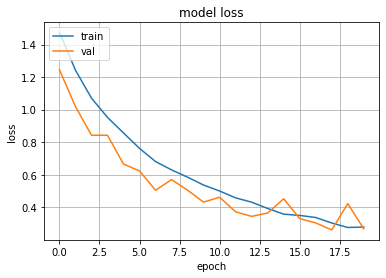
\includegraphics[scale = 0.5]{CHAPTERS/Chapter-4/Images/4.6b}}
        \caption{Training \& validation loss}
        \label{fig:4.4b}
    \end{subfigure}
    \caption[]{Model accuracy \& model loss}
    \label{fig:4.6}
  \end{figure}
  The loss was categorical\_crossentropy in this case. 
  The training accuracy recorded after 20 epochs was 90.2\% and training
  loss was 0.2778. The test set was choosen as validation data and
  validation accuracy after 20 epochs 
  was 90.16\% and validation loss was 0.2675.
  The values of training
  and validation accuracy \& training and validation loss
  against number of epochs for five class vehicle classifier
  are tabulated in Table \ref{table:4.2}.

\begin{table}[H]
    \caption{Results for binary class vehicle classifier}
    \label{table:4.2}
	  \begin{center}
		\scalebox{0.85}
		{\begin{tabular}{|l |l |l |l |l |l |}
		\hline
		S.No & Number of epochs & Training accuracy & Validation accuracy & Training loss & Validation loss\\ \hline
		1  & 5 & 0.6689 & 0.7644 & 0.8381 & 0.6587
		\\ \hline
		2  & 10 & 0.8253 & 0.8680 & 0.4851 & 0.3689
        \\ \hline %
        3   & 15 &  0.8741 & 0.8928  &0.3639  & 0.3084
        \\ \hline %
        4   & 20 &  0.9020 & 0.9016  &0.2778  & 0.2675
        \\ \hline %
		\end{tabular}}
	  \end{center}
\end{table}

\section{Graphical User Interface}
In order to observe the results visually we have developed a Graphical User
Interface (GUI) using tkinter package of 
Python. The test images are given as inputs to our trained
model one-by-one and corresponding labels are generated.
Since we cannot run tkinter on Google Colab,
so we saved our trained model in the local disk of our computer.
To visually display the testing results, all the images in the test dataset are used as inputs to the trained model that we have loaded  from our workspace
and the predicted class labels are displayed on the GUI accordingly.
Some examples are shown in
figure \ref{fig:4.7}.

\begin{figure}[htbp]
    \centering
    \begin{subfigure}[t]{0.3\textwidth}
        \fbox{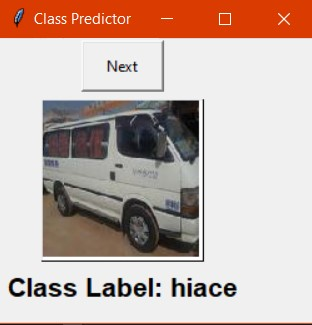
\includegraphics[width = 4.5cm, height = 4.5cm]{CHAPTERS/Chapter-4/Images/4.7a}}
        \caption{}
        \label{fig:4.7a}
    \end{subfigure}
    \begin{subfigure}[t]{0.3\textwidth}
        \fbox{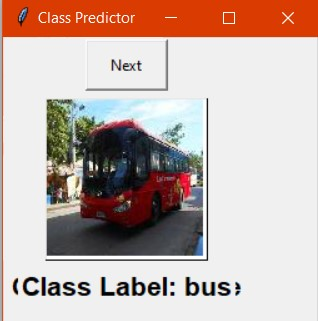
\includegraphics[width = 4.5cm, height = 4.5cm]{CHAPTERS/Chapter-4/Images/4.7b}}
        \caption{}
        \label{fig:4.7b}
    \end{subfigure}
    \begin{subfigure}[t]{0.3\textwidth}
      \fbox{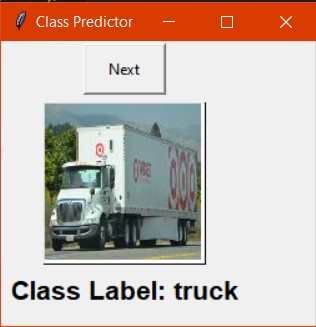
\includegraphics[width = 4.5cm, height = 4.5cm]{CHAPTERS/Chapter-4/Images/4.7c}}
      \caption{}
      \label{fig:4.7c}
  \end{subfigure}
    \captionsetup{justification = centering}
    \caption[]{Test images and labels on a GUI}
    \label{fig:4.7}
  \end{figure}

\section{Limitations \& Future Work}

For binary classification problem, the proposed model does not work on high resolution images.
Processing high resolution imagery might be a requirement in biomedical imaging,
since changing resolution might change the
local and global parameters content in the image. For high resolution images, we use Res-Net architecture which is complex and
requires high computational power. We have used a variant of VGG-16 for
our five class problem. Highly complex model may cause overfitting.
For future work, the detailed study
about tuning of hyperparameters is included.
Problem of overfitting can be eliminated by performing an
extensive search over hyper-parameters space to obtain optimum 
values of these parameters for our model.
Hyper-parameters include, no of convolutional layers, layer filters,
filter depth, pooling type, activation functions, length and number
of dense layers, drop-outs, batch-size,epochs, optimizers and loss
functions etc.
